\documentclass{article}
\usepackage{fontawesome}        % faKeyboard faSuitcase faWrench
\usepackage{lmodern}            % Smoothly scaling font.
\usepackage[                    % Set the default font size.
fontsize=24,
]{fontsize}
\renewcommand{\familydefault}{\sfdefault}
\usepackage[
% - HP DesignJet Z5200 printer in the Chemical Engineering department
%   has a 42" roll width (1067 mm).
% - The FacultyHack @ Science Gateways 2025 conference allows 30"x45"
% - Therefore, crop the poster to 42in height i.e. 30"x42"
paperwidth=30in,
paperheight=42in,
margin=0.5cm,
head=2.17in,
foot=1.89in,
includeheadfoot,
%showframe,
]{geometry}
\usepackage{fancyhdr}
\title{GPUs for massively parallel mechanistic modeling}
\pagestyle{fancy}
\renewcommand{\headrulewidth}{0pt}
\renewcommand{\footrulewidth}{0pt}
\fancyhead[L]{%
  \begin{tikzpicture}[%
    background rectangle/.style = {
      fill = fh-blue,
    },
    show background rectangle,
    tight background,
    scale = 1]
    \node (ref) [
    minimum width = \paperwidth - 1cm,
    minimum height = 2.47in] {};
    \node at (ref.north west) [anchor = north west, name = fh] {%
      
\includegraphics[height=2.47in]{fh.png}};
    \node at (ref.south east) [%
    anchor = south east, %
    name = nsf-text,
    text = fh-gold,
    scale = 0.5,
    inner sep = 6pt,
    text width = width("under award number 2231406"),
    align = center] {%
      SGX3 is funded by the \mbox{National Science Foundation} %
      under award number 2231406};
    \path let
    \p1 = (ref.north),
    \p2 = (nsf-text.north),
    \n1 = {(\y1 - \y2) - 4pt} in
    node at (nsf-text.north) [anchor = south, name = nsf, yshift = -2pt] {%
      \includegraphics[height=\n1]{NSF_Official_logo_RGB.eps}};
    \node at (fh.east) [%
    anchor = west,
    text = fh-gold,
    scale = 3,
    text width = width("GPUs for massively parallel")] {%
      GPUs for massively parallel mechanistic modeling%
    };
  \end{tikzpicture}%
}
\fancyhead[C,R]{}
\fancyfoot[L]{%
  \begin{tikzpicture}[%
    background rectangle/.style = {
      fill = fh-blue,
      inner sep = 0pt,
    },
    show background rectangle,
    tight background,
    scale = 1]
    \pgfdeclarelayer{foreground}
    \pgfsetlayers{background,main,foreground}
    \begin{pgfonlayer}{foreground}
    \node (ref) [
    inner sep = 0,
    minimum width = 30in - 1cm,
    minimum height = 1.59in] {};
    \node (sgx3) at ([xshift=0.5cm]ref.west) [anchor = west] {%
      
\includegraphics[height=0.85in]{sgx3.png}};
    \node (ornl) at (sgx3.east) [anchor = west] {%
      
\includegraphics[height=1.04in]{ornl.png}};
    \node (omnibond) at (ornl.east) [anchor = west] {%
      
\includegraphics[height=0.87in]{omnibond.jpg}};
    \node (tacc) at (omnibond.east) [anchor = west] {%
      
\includegraphics[height=0.87in]{tacc.png}};
    \node (qr-code) at (ref.east) [anchor = east, outer sep = 0.25cm] {%
      
\includegraphics[height=1.32in]{qr-code.png}};
    \node at (qr-code.west) [anchor = east, text = fh-gold, scale = 1.6] {%
      \textbf{Event Site:} %
      \url{https://hackhpc.github.io/facultyhack-gateways25}
      };
    \end{pgfonlayer}
    \begin{pgfonlayer}{main}
      \node [
      inner sep = 0pt, fit = (sgx3) (ornl) (omnibond) (tacc), fill = white] {};
    \end{pgfonlayer}
  \end{tikzpicture}%
}
\fancyfoot[C]{}

\usepackage{graphicx}
\graphicspath{{img/}}

\usepackage{multicol}
\setlength{\columnseprule}{0pt}
\setlength{\columnsep}{2.5pc}

\usepackage{tikz}
\usepackage{tikz}
\tikzset{
  every node/.style = {
    inner sep = 0pt,
    outer sep = 0pt
  }
}
\usetikzlibrary{
arrows.meta,
backgrounds,
calc,
decorations.markings,
decorations.pathmorphing,
decorations.text,
fit,
mindmap,
tikzmark
}

\usepackage{soul}

\usepackage{amssymb}            % \blacksquare
\usepackage{amsmath}            % \text

\usepackage{tabularx}
\newcolumntype{C}{>{\centering\arraybackslash}X}
\newcolumntype{R}{>{\raggedleft\arraybackslash}X}
% Vertically center within row https://tex.stackexchange.com/a/343329
\renewcommand\tabularxcolumn[1]{m{#1}}
\usepackage{booktabs}
\usepackage{multirow}

\usepackage[
abbreviate=true,
bibencoding=utf8,
minnames=2,
maxbibnames=99,
sorting=none,
style=vancouver,
citestyle=numeric-comp,
url=false,
]{biblatex}
% The vancouver citation style is based on NLM per
% https://tex.stackexchange.com/a/371433
\addbibresource{references.bib}
\renewcommand*{\bibfont}{\scriptsize\selectfont}

\usepackage[
table
]{xcolor}
\definecolor{fh-blue-lighter}{HTML}{EBEFF7}
\definecolor{fh-blue-darker}{HTML}{D4DEED}
\definecolor{fh-blue}{RGB}{0,89,157}
\definecolor{fh-gold}{HTML}{F7E8C9}

\usepackage{tcolorbox}
\tcbuselibrary{poster}
\newcommand{\sectionbox}[1]{%
  \begin{tcolorbox}[sharp corners,boxrule=0pt,top=15pt,colback=fh-blue,coltext=fh-gold]%
    \section*{#1\vphantom{Yy}}%
  \end{tcolorbox}%
}

% Reduce excessive hyphenation https://stackoverflow.com/a/65156105
\tolerance=9999
\emergencystretch=10pt
\hyphenpenalty=10000
\exhyphenpenalty=100

\begin{document}

\noindent
\begin{tcbposter}[
  poster = {
    rows = 1,
    columns = 2,
    height = \paperheight - 2cm - 2.47in - 1.59in,
    width = \paperwidth - 1cm,
    colspacing = 0.1in,
    rowspacing = 0.1in,
    %showframe,
  },
  boxes = {
    fonttitle = \Large\bfseries,
    coltitle = fh-gold,
    colbacktitle = fh-blue,
    colback = white,
    colframe = white,
    sharp corners,
    boxrule = 0pt,
  },
  ]

  \posterbox[
  adjusted title = Introduction,
  ]{
    name = intro,
    column = 1,
  }{%
  \noindent
  Graphical Processing Units (GPUs) %
  are integrated into the core architecture %
  of the world's fastest supercomputers %
  that solve the most computationally difficult, %
  mechanistic scientific problems.
  %
  An 8~year, \$1.8~billion effort %
  called the Exascale Computing Project (ECP) %
  involving 2,800 scientists and engineers %
  recently finished modernizing %
  the underlying scientific numerical software %
  to efficiently use this new generation of machines.
  \smallskip

  \noindent
  Computing facilities grant access at no cost %
  to these GPU-accelerated%
  \supercite{%
    carter_2014,%
    beckingsale_2019,%
    reinders_2023%
  } machines %
  only to research software engineers and scientists who demonstrate that %
  their computations scale %
  to efficiently use multiple GPUs across many computer servers / nodes.
  %
  Therefore, %
  it is imperative to teach %
  the data parallel software development skills, %
  appropriate domain science methods, and %
  sustainable software practices %
  to enable large scale, GPU-centric computational research.
  %
  Discussion and feedback on this poster from the community %
  can help make this course a success and %
  support similar hands-on learning and teaching endeavors.
  \smallskip

  \noindent
  \begin{minipage}[c]{.3\linewidth}
    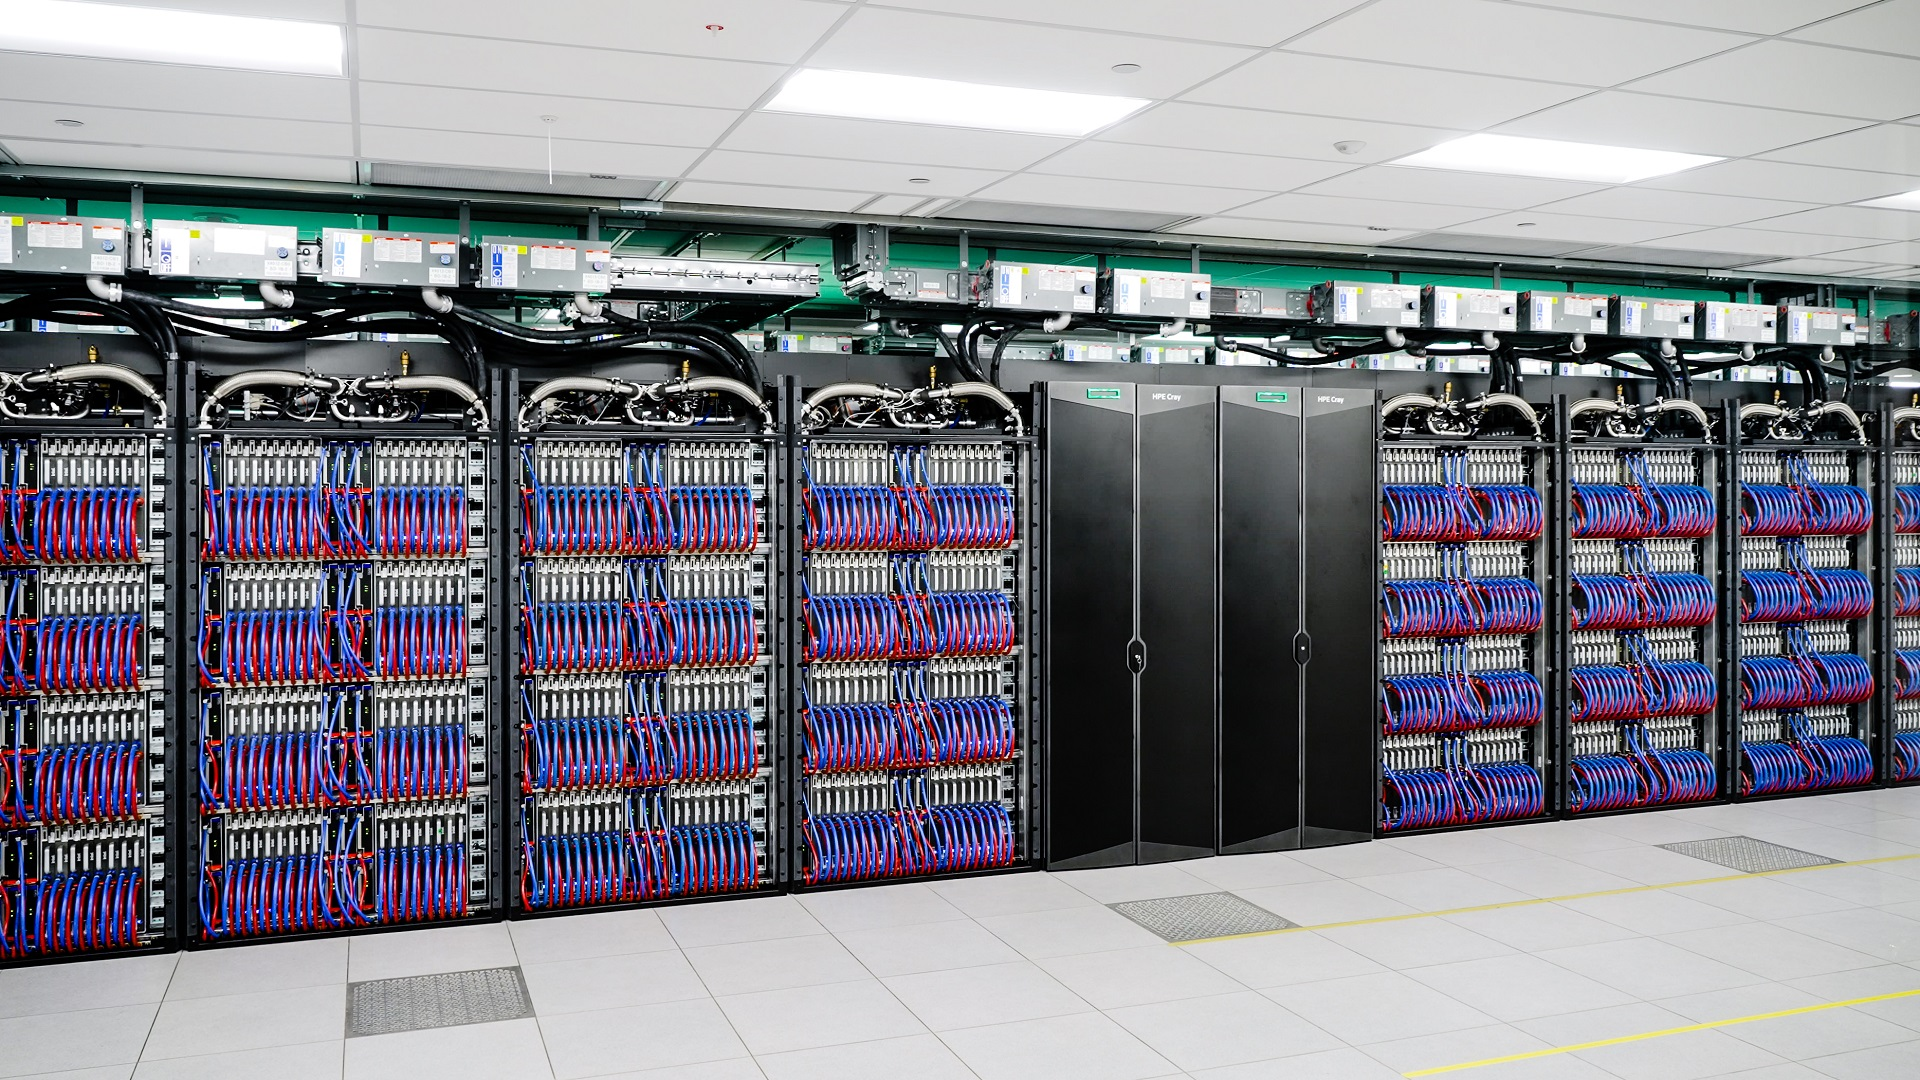
\includegraphics[width=\linewidth]{1920x1080-Aurora hero image.jpg}
  \end{minipage}
  \begin{minipage}[c]{.7\linewidth}
    \textbf{Modern supercomputers use GPU architectures.}
    %
    Left photo is the Aurora supercomputer at Argonne National Laboratory %
    that is ranked 3\textsuperscript{rd} in the Top 500 List of June 2025 %
    and one of three US exascale supercomputers.
    %
    Germany recently launched their first exascale supercomputer, JUPITER, %
    and China may have as many as 10 exascale supercomputers %
    by the end of this year\supercite{dongarra_2023} %
    but stopped submitting data to the Top 500 List %
    after US GPU embargoes.
  \end{minipage}

  \vspace{-.5\baselineskip}
  \subsection*{\textcolor{fh-blue}{Target Course Description}}
  \vspace{-.5\baselineskip}
  {
    \rowcolors{1}{fh-blue-lighter}{fh-blue-darker}
    \begin{tabularx}{\linewidth}{>{\bfseries}r X}
      \toprule
      Course Name:
      & GPUs for massively parallel mechanistic modeling\\
      Course Number:
      & TBA\\
      Department:
      & Chemical Engineering\\
      Anticipated Enrollment:
      & 12\\
      Prerequisites:
      & fluent with at least one %
      procedural programming language\\
      Key Content:
      & performance optimization, %
      software development, %
      domain science methods, %
      capstone project\\
      Description:
      & This course trains graduate researchers %
      with ECP-level skills in high performance computing (HPC), %
      using research software engineer (RSE) rigor, %
      and HPC-relevant domain scientific methods.\\
      Project Repo:
      & \small \url{https://github.com/omsai/facultyhack-gateways25-nanda}\\
      \bottomrule
    \end{tabularx}
  }

  \vspace{-\baselineskip}
  \subsection*{\textcolor{fh-blue}{Goals}}
  \vspace{-.5\baselineskip}
  \begin{itemize}
  \setlength{\itemsep}{-.5em}
  \item Setup student \ul{JetStream2 VM} for homework and capstone projects.
  \item Add students to my \ul{ACCESS group} for cluster runs and %
    help them get their own ACCESS allocation.
  \item Teach all C++ classroom exercises inside a \ul{web IDE}.
  \item Train students to \ul{package their project}.
  \end{itemize}
  }

  \posterbox[
  adjusted title = Initial Course Syllabus,
  ]{
    name = syl-init,
    column = 1,
    below = intro,
  }{%
  \noindent
  This course was inspired by the %
  2024 Argonne Training Program on Extreme-Scale Computing (ATPESC'24) %
  and the 2025 LLNL %
  High Performance Computing Innovation Center (HPC-IC'25) %
  tutorial series.
  \medskip

    \noindent
    \begin{tabularx}{\linewidth}{%
      >{\hsize=.18\hsize\linewidth=\hsize}X %
      >{\hsize=.33\hsize\linewidth=\hsize}R %
      >{\hsize=.15\hsize\linewidth=\hsize}C %
      >{\hsize=.15\hsize\linewidth=\hsize}C %
      >{\hsize=.15\hsize\linewidth=\hsize}C}
      \toprule
      \textbf{Category}
      & \textbf{Topic}
      & \textbf{This Course} & \textbf{ATPESC'24} & \textbf{HPC-IC'25}\\
      \midrule
      \multirow{4}{\hsize}{\textcolor{orange!90!black}{$\blacksquare$}
      Performance \phantom{$\blacksquare$}~optimization}
      & Within node
      & \checkmark & \checkmark & $\times$\\
      & Multi-node
      & \checkmark & \checkmark & \checkmark\\
      & GPU performance portability
      & \checkmark & \checkmark & \checkmark\\
      & Performance tuning
      & \checkmark & \checkmark & \checkmark\\
      \midrule
      \multirow{6}{\hsize}{\textcolor{blue!80!black}{$\blacksquare$}
      Software \phantom{$\blacksquare$}~development}
      & Unit testing
      & \checkmark & \checkmark & $\times$\\
      & Performance testing
      & \checkmark & \checkmark & \checkmark\\
      & CI, checkpointing, benchmarking
      & \checkmark & $\times$ & \checkmark\\
      & Parallel debugging
      & \checkmark & \checkmark & $\times$\\
      & Code peer review, documentation
      & \checkmark & $\times$ & $\times$\\
      & Packaging
      & \checkmark & \checkmark & \checkmark\\
      \midrule
      \multirow{-0.5}{\hsize}{\textcolor{green!50!black}{$\blacksquare$}
      Domain science \phantom{$\blacksquare$}~methods}
      & Mechanistic multiscale modeling
      & \checkmark & $\times$ & $\times$\\
      & Scientific parameter fitting
      & \checkmark & $\times$ & $\times$\\
      & Coupling AI, cloud, data science
      & \checkmark & $\times$ & \checkmark\\
      \midrule
      \multirow{2}{\hsize}{\textcolor{black!60}{$\blacksquare$}
      Sysadmin}
      & Cluster launch
      & \checkmark & $\times$ & \checkmark\\
      & Cluster profiling
      & \checkmark & \checkmark & \checkmark\\
    \end{tabularx}
  }

  \posterbox[
  adjusted title = Mentors Suggestions,
  ]{
    name = sugg,
    column = 1,
    below = syl-init,
  }{%
  \begin{multicols}{2}
    \begin{enumerate}
    \setlength{\itemsep}{0em}
    \item \ul{Added network communication exercises} %
      using the LAMMPS exercise developed at Temple University.
    \item \ul{Added profiling exercises} %
      from Cornell University %
      and the University of Michigan.
    \item \ul{Chose a checkpointing library} %
      written in C++ %
      both to teach in the course %
      and to recommend for student capstone projects.
    \item Trainees will \ul{write C++ code using VS Code} %
      with SSH tunnels to JetStream2 virtual machines %
      with a fallback of OpenVSCode Server web interface %
      for classroom instruction.
    \item \ul{Added AI policy} %
      requiring a bibliography %
      citing AI service names with versions, prompts, and output.
    \item Moved non-capstone homework assignments to %
      \ul{classroom hands-on to avoid over-reliance on AI support} %
      while trainees are still developing expertise.
    \item \ul{Increased accessibility} %
      for non-C++ programmers %
      by recommending self-guided, open access textbooks %
      from \emph{The Art of HPC: Volume 3}.
    \item \ul{Added objective of numerical correctness} %
      but limited goal to unit tests, performance test, and CI %
      instead of considering formal methods.
    \item The target audience is now \ul{graduate students} %
      with existing projects or pilot projects.
    \item \ul{Consolidated course topics} %
      to focus on domain science methods %
      in keeping with the course title.
    \end{enumerate}
  \end{multicols}
  }

  \posterbox[
  adjusted title = Science Gateways Resources Used,
  ]{
    name = res,
    column = 1,
    below = sugg,
  }{%
  \begin{multicols}{2}
    \begin{tikzpicture}
      \node (text) %
      [text width = .7\linewidth] {%
        \textbf{Non-virtual multi-GPU A100 nodes (g3.2xl)}};
      \node (logo) at (text.south east) %
      [anchor = south west, minimum width = .3\linewidth] {%
        
\includegraphics[width=.3\linewidth]{jetstream2-head-logo.pdf}};
    \end{tikzpicture}
    \vspace{-1.5\baselineskip}
    \begin{itemize}
    \setlength{\itemsep}{-.5em}
    \item Shared between small groups of 4 students.
    \item For early project development and exercises.
    \item A100 supports 64-bit floating point operations %
      for capstone projects that may require it.
    \item Efficient multi-GPU use is a course objective.
    \item g3.2xl is the multi-GPU A100 with the most availability.
    \end{itemize}

    \begin{tikzpicture}
      \node (text) %
      [text width = .7\linewidth] {%
        \textbf{Bridges-2 GPU HPC allocation}};
      \node (logo) at (text.south east) %
      [anchor = south west, minimum width = .3\linewidth] {%
        
\includegraphics[width=.3\linewidth]{access-logo.pdf}};
    \end{tikzpicture}
    \vspace{-1.5\baselineskip}
    \begin{itemize}
    \setlength{\itemsep}{-.5em}
    \item For cluster exercises and scaling.
    \item Interactive nodes with backfill scheduling and short walltime %
    for the classroom use.
    \item Trainees are encouraged %
    to apply for their own ACCESS CI allocations %
    to continue their work %
    after leaving the instructor's ACCESS CI group.
    \end{itemize}

    \begin{tikzpicture}
      \node (text) %
      [text width = .7\linewidth] {%
        \textbf{HPC introduction and reproducible workflows}};
      \node (logo) at (text.south east) %
      [anchor = south west, minimum width = .3\linewidth] {%
        
\includegraphics[width=.3\linewidth]{hpc-carpentry.pdf}};
    \end{tikzpicture}
    \vspace{-1.5\baselineskip}
    \begin{itemize}
    \setlength{\itemsep}{-.5em}
    \item Self-paced introduction to key concepts of the  HPC environment.
    \item Supplementary reading for %
      capstone project reproducible workflows %
      for coupling AI, cloud, and data science tools.
    \end{itemize}

    \begin{tikzpicture}
      \node (text) %
      [text width = .8\linewidth] {%
        \textbf{%
          Trainee GitHub repositories for assignments and capstone projects}};
      \node (logo) at (text.south east) %
      [anchor = south west, minimum width = .2\linewidth] {%
        
\includegraphics[width=.1\linewidth]{github-mark.pdf}
        
\includegraphics[width=.1\linewidth]{actions-icon-actions.pdf}
      };
    \end{tikzpicture}
    \vspace{-1.5\baselineskip}
    \begin{itemize}
    \setlength{\itemsep}{-.5em}
    \item Projects in private git repositories shared with the instructor.
    \item Assignments partially checked using GitHub actions.
    \item Progress on capstone projects will be monitored from git repositories.
    \end{itemize}
  \end{multicols}
  }

  \posterbox[
  adjusted title = Modified Course Syllabus,
  ]{
    name = syl-modified,
    column = 2,
  }{%
    Each node corresponds to about %
    one week of semester classroom sessions.
    %
    Key: %
    \faSuitcase{} = standalone homework, %
    \faWrench{} = capstone homework, %
    \faKeyboardO{} = classroom hands-on exercise, %
    * = optional lecture that may be dropped %
    to review previous, critical lectures.
    \begin{center}
    \vspace{-\baselineskip}
    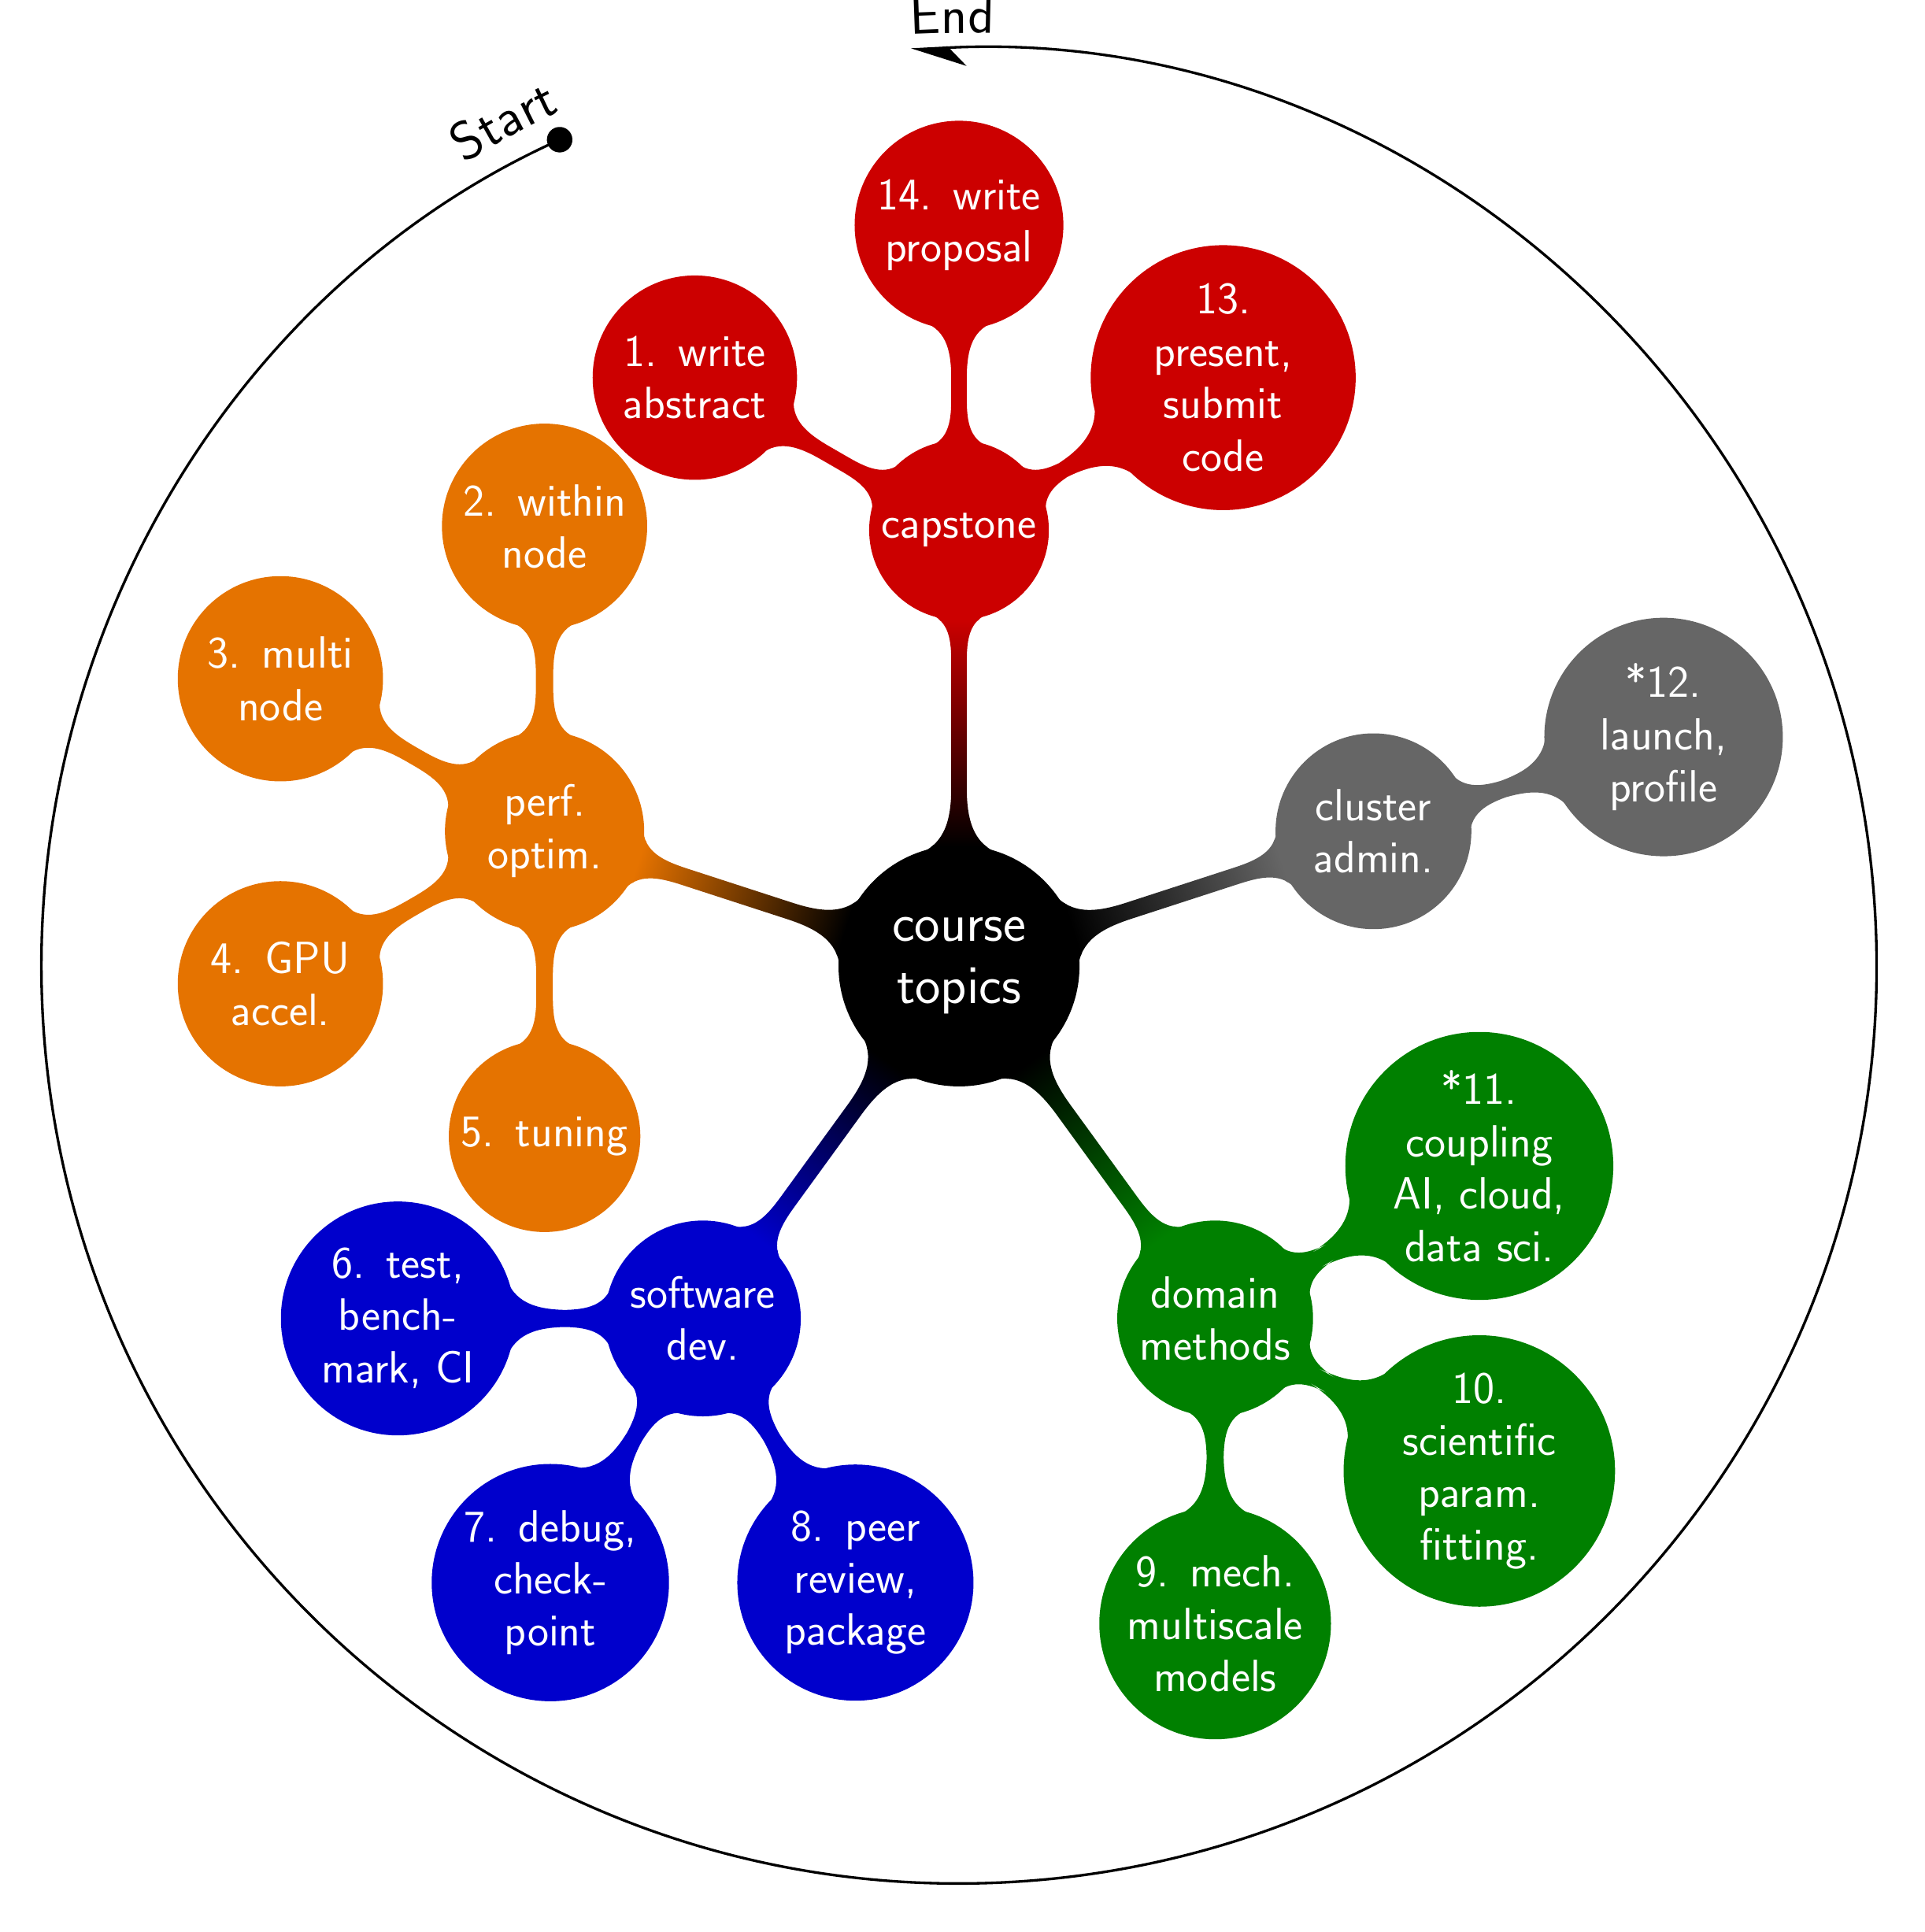
\begin{tikzpicture}[
      root concept/.style={
        text width = 100pt,
      },
      level 1 concept/.style={
        text width = 80pt,
        level distance = 200,
        font = \footnotesize,
      },
      level 2 concept/.append style={
        text width = 85pt,
        level distance = 140,
        font = \footnotesize,
      },
      mindmap,
      ]
      \path
      node [concept, concept color=black, text=white, name=node-concept]
      {course topics}
      child [grow=90, concept color=red!80!black, text=white] {
        node [concept] {capstone}
        [clockwise from=150]
        child { node [concept] {1. write abstract} }
        child { node [concept, name=node-proposal] {14. write proposal} }
        child { node [concept] {13. present, submit code} }
      }
      child [grow=162, concept color=orange!90!black, text=white] {
        node [concept] {perf. optim.}
        [counterclockwise from=90]
        child { node [concept] {2. within node} }
        child { node [concept] {3. multi node} }
        child { node [concept] {4. GPU accel.} }
        child { node [concept] {5. tuning} }
      }
      child [grow=234, concept color=blue!80!black, text=white] {
        node [concept] {software dev.}
        [counterclockwise from=180]
        child { node [concept] {6. test, benchmark, CI} }
        child { node [concept] {7. debug, checkpoint} }
        child { node [concept] {8. peer review, package} }
      }
      child [grow=306, concept color=green!50!black, text=white] {
        node [concept] {domain methods}
        [counterclockwise from=270]
        child { node [concept] {9. mech. multiscale models} }
        child { node [concept] {10. scientific param. fitting.} }
        child { node [concept] {*11. coupling AI,~cloud, data sci.} }
      }
      child [grow=18, concept color=black!60, text=white] {
        node [concept] {cluster admin.}
        [clockwise from=18]
        child { node [concept, name=node-cluster] {*12. launch, profile} }
      };
      \draw [%
      very thick,
      {Stealth[harpoon,length=1em]-Circle[length=0.5em]},
      postaction={
        decorate,
        decoration={
          text align={left},
          raise={0.3em},
          text along path,
          text={End}
        }
      },
      postaction={
        decorate,
        decoration={
          text align={right},
          raise={0.5em},
          text along path,
          text={Start}
        }
      }]
      ([shift=(93:18em)]node-concept) arc (93:-245:18em);
    \end{tikzpicture}
    \end{center}
    \vspace{-2\baselineskip}
    \begin{multicols}{2}
      \begin{enumerate}
      \item \textcolor{red!80!black}{\faWrench{}}
        Write a half page proposal for a new or
        existing compute-intensive mechanistic model to be accelerated
        using GPU resources.%
      \item \textcolor{orange!90!black}{\faSuitcase{}}
        Vectorize Python code,
        inspect C assembler CPU vectorized instructions, create
        roofline plots to inspect CPU-memory, inspect memory
        hierarchy.%
      \item \textcolor{orange!90!black}{\faSuitcase{}}
        TaskWorks, Spack, MPI, and SLURM.%
      \item \textcolor{orange!90!black}{\faSuitcase{}}
        C++ Kokkos to fill in
        the blanks of partially completed programs.\\
        \textcolor{orange!90!black}{\faWrench{}}
        Outline capstone project goals and objectives
        with rough semester timeline.%
      \item \textcolor{orange!90!black}{\faSuitcase{}}
        Darashan, Drishti, and
        HPCtoolkit.\\
        \textcolor{orange!90!black}{\faWrench{}}
        Literature review of software
        similar to yours and how you intend to make yours different.%
      \item \textcolor{blue!80!black}{\faKeyboardO{}}
        PyTest, Benchpark, and
        Jacamar CI.\@\\
        \textcolor{blue!80!black}{\faWrench{}}
        Start adding tests, coverage, benchmarks,
        and continuous integration.%
      \item \textcolor{blue!80!black}{\faKeyboardO{}}
        Peer pairing.\\
        \textcolor{blue!80!black}{\faWrench{}}
        Document, package with Spack or Apptainer.%
      \item \textcolor{blue!80!black}{\faKeyboardO{}}
        MPIGDB debugging session, resuming from
        checkpoint
        to understand error, correctness with sanitizers.\@\\
        \textcolor{blue!80!black}{\faWrench{}}
        Start adding checkpointing.%
      \item \textcolor{green!50!black}{\faKeyboardO{}}
        Analyze how model layers and linking are
        implemented\supercite{cilfone_2015}.%
      \item \textcolor{green!50!black}{\faKeyboardO{}}
        Calibrating our model from last time with
        pyabc using adaptive sampling; discuss
        checkpointing, debugging.\\
        \textcolor{green!50!black}{\faWrench{}}
        Start coupling with scientific parameter sampling.%
      \item \textcolor{green!50!black}{\faSuitcase{}}
        Summarize book\supercite{zbakh_2024} chapters 4
        and 8 in 1 page.\\
        \textcolor{green!50!black}{\faWrench{}}
        Assess possible extensions using components of AI, big data, or
        cloud applications and specialized hardware needs with your
        domain science, and to what extent we discussed these concepts
        so far in the class.%
      \item \textcolor{black!60}{\faKeyboardO{}}
        Setup VMs with network, shared disk, and
        SLURM to launch and profile an ad-hoc, suboptimal cluster
        to compare with a professionally architected and tuned cluster.%
      \item \textcolor{red!80!black}{\faKeyboardO{}}
        Walk though your project with
        ACCESS-relevant details and future directions.\\
        \textcolor{red!80!black}{\faWrench{}} Submit code for grading.%
      \item \textcolor{red!80!black}{\faWrench{}}
        Write a 3-page ACCESS CI
        Accelerate proposal with scaling studies and justification for
        compute resources; trim actual Discover proposal to
        1-page.%
      \end{enumerate}
    \end{multicols}
  }

  \posterbox[
  adjusted title = Expansions,
  ]{
    name = exp,
    column = 2,
    below = syl-modified,
  }{%
  \begin{multicols}{2}
    \begin{enumerate}
    \setlength{\itemsep}{0em}
    \item Accommodate \ul{undergraduate students} %
      with more structure, %
      shorter exercises, %
      and allow them to choose from a set of smaller capstone projects.
    \item For the last ``fun'' topic before final presentations %
      \ul{launch the cluster using Raspberry Pis}, %
      networking hardware, and network storage %
      for a more memorable hands-on lesson.
    \item Develop an \ul{time-saving exercise for model comparison} %
      to demonstrate the usefulness %
      of detailed benchmarking and analysis tools %
      \ul{to rapidly iterate model development}.
    \item Create \ul{interactive trivial exercises in a web page} %
      to encourage trainee progress with %
      a live updating grading rubric %
      and suggestions to correct common errors.
    \item \ul{Compartmentalize topics %
      into the 2-day workshop format} %
      to be taught at the Pittsburgh Supercomputing Center (PSC).
    \item Create \ul{HPC Carpentry lessons in C++ for data scientists}
      to cover C++ concepts required to use GPU performance
      portability libraries by comparing to concepts in Python and R
      where possible, namely: variables, functions, data structures,
      loops, classes (constructors, member variables, member
      functions, member operators), debugging.
    \end{enumerate}
  \end{multicols}
  }

  \posterbox[
  adjusted title = References,
  ]{
    name = references,
    column = 2,
    below = exp,
  }{%
  {
    % Recalculate \columnsep instead of using the large \columnsep
    % from the main document.
    \setlength{\columnsep}{1.5pc}
    \begin{multicols}{2}
      \printbibliography[heading=none]{}
    \end{multicols}
  }
  }

  \posterbox[
  adjusted title = Authors,
  ]{
    name = authors,
    column = 2,
    below = references,
  }{%
    \vspace{-.1\baselineskip}
  \begin{tikzpicture}
    \node (pn) {%
    \includegraphics[%
    keepaspectratio,
    width=10em,
    height=4.6em,
    clip,
    trim={55 85 50 35}]{%
        pariksheet.png}};

    \node (pn-text) at (pn.north east) [anchor = north west, xshift = 0.5em, align = left] {%
      \textcolor{fh-blue}{\tikzmark{pn}Nanda, Pariksheet}\\
      Role: Faculty Participant\\
      University of Pittsburgh\\
      pan79@pitt.edu
    };

    \node (em) at ($ (pn.north west) + (.5\linewidth,0) $) [%
    anchor = north west,
    xshift = 1em] {%
      \includegraphics[%
      keepaspectratio,
      width=10em,
      height=4.6em,
      clip,
      trim={20 80 60 5}]{%
        elijah.jpg}};

    \node at (em.north east) [anchor = north west, xshift = 0.5em, align = left] {%
      \textcolor{fh-blue}{\tikzmark{pn}MacCarthy, Elijah}\\
      Role: Community Mentor\\
      Oak Ridge National Laboratory\\
      maccarthyea@ornl.gov
    };
  \end{tikzpicture}
  }

\end{tcbposter}

\end{document}
